% GNUPLOT: LaTeX picture with Postscript
\begingroup
  \makeatletter
  \providecommand\color[2][]{%
    \GenericError{(gnuplot) \space\space\space\@spaces}{%
      Package color not loaded in conjunction with
      terminal option `colourtext'%
    }{See the gnuplot documentation for explanation.%
    }{Either use 'blacktext' in gnuplot or load the package
      color.sty in LaTeX.}%
    \renewcommand\color[2][]{}%
  }%
  \providecommand\includegraphics[2][]{%
    \GenericError{(gnuplot) \space\space\space\@spaces}{%
      Package graphicx or graphics not loaded%
    }{See the gnuplot documentation for explanation.%
    }{The gnuplot epslatex terminal needs graphicx.sty or graphics.sty.}%
    \renewcommand\includegraphics[2][]{}%
  }%
  \providecommand\rotatebox[2]{#2}%
  \@ifundefined{ifGPcolor}{%
    \newif\ifGPcolor
    \GPcolorfalse
  }{}%
  \@ifundefined{ifGPblacktext}{%
    \newif\ifGPblacktext
    \GPblacktexttrue
  }{}%
  % define a \g@addto@macro without @ in the name:
  \let\gplgaddtomacro\g@addto@macro
  % define empty templates for all commands taking text:
  \gdef\gplfronttext{}%
  \gdef\gplfronttext{}%
  \makeatother
  \ifGPblacktext
    % no textcolor at all
    \def\colorrgb#1{}%
    \def\colorgray#1{}%
  \else
    % gray or color?
    \ifGPcolor
      \def\colorrgb#1{\color[rgb]{#1}}%
      \def\colorgray#1{\color[gray]{#1}}%
      \expandafter\def\csname LTw\endcsname{\color{white}}%
      \expandafter\def\csname LTb\endcsname{\color{black}}%
      \expandafter\def\csname LTa\endcsname{\color{black}}%
      \expandafter\def\csname LT0\endcsname{\color[rgb]{1,0,0}}%
      \expandafter\def\csname LT1\endcsname{\color[rgb]{0,1,0}}%
      \expandafter\def\csname LT2\endcsname{\color[rgb]{0,0,1}}%
      \expandafter\def\csname LT3\endcsname{\color[rgb]{1,0,1}}%
      \expandafter\def\csname LT4\endcsname{\color[rgb]{0,1,1}}%
      \expandafter\def\csname LT5\endcsname{\color[rgb]{1,1,0}}%
      \expandafter\def\csname LT6\endcsname{\color[rgb]{0,0,0}}%
      \expandafter\def\csname LT7\endcsname{\color[rgb]{1,0.3,0}}%
      \expandafter\def\csname LT8\endcsname{\color[rgb]{0.5,0.5,0.5}}%
    \else
      % gray
      \def\colorrgb#1{\color{black}}%
      \def\colorgray#1{\color[gray]{#1}}%
      \expandafter\def\csname LTw\endcsname{\color{white}}%
      \expandafter\def\csname LTb\endcsname{\color{black}}%
      \expandafter\def\csname LTa\endcsname{\color{black}}%
      \expandafter\def\csname LT0\endcsname{\color{black}}%
      \expandafter\def\csname LT1\endcsname{\color{black}}%
      \expandafter\def\csname LT2\endcsname{\color{black}}%
      \expandafter\def\csname LT3\endcsname{\color{black}}%
      \expandafter\def\csname LT4\endcsname{\color{black}}%
      \expandafter\def\csname LT5\endcsname{\color{black}}%
      \expandafter\def\csname LT6\endcsname{\color{black}}%
      \expandafter\def\csname LT7\endcsname{\color{black}}%
      \expandafter\def\csname LT8\endcsname{\color{black}}%
    \fi
  \fi
    \setlength{\unitlength}{0.0500bp}%
    \ifx\gptboxheight\undefined%
      \newlength{\gptboxheight}%
      \newlength{\gptboxwidth}%
      \newsavebox{\gptboxtext}%
    \fi%
    \setlength{\fboxrule}{0.5pt}%
    \setlength{\fboxsep}{1pt}%
\begin{picture}(5000.00,5000.00)%
    \gplgaddtomacro\gplfronttext{%
      \colorrgb{0.15,0.15,0.15}%
      \put(518,3702){\makebox(0,0)[r]{\strut{}\small $10\texttt{e}$$-$$4$}}%
      \colorrgb{0.15,0.15,0.15}%
      \put(518,4009){\makebox(0,0)[r]{\strut{}\small $10\texttt{e}$$-$$3$}}%
      \colorrgb{0.15,0.15,0.15}%
      \put(518,4317){\makebox(0,0)[r]{\strut{}\small $10\texttt{e}$$-$$2$}}%
      \colorrgb{0.15,0.15,0.15}%
      \put(518,4624){\makebox(0,0)[r]{\strut{}\small $10\texttt{e}$$-$$1$}}%
      \colorrgb{0.15,0.15,0.15}%
      \put(771,3482){\makebox(0,0){\strut{}}}%
      \colorrgb{0.15,0.15,0.15}%
      \put(1376,3482){\makebox(0,0){\strut{}}}%
      \colorrgb{0.15,0.15,0.15}%
      \put(1982,3482){\makebox(0,0){\strut{}}}%
      \colorrgb{0.15,0.15,0.15}%
      \put(2587,3482){\makebox(0,0){\strut{}}}%
      \colorrgb{0.15,0.15,0.15}%
      \put(3192,3482){\makebox(0,0){\strut{}}}%
      \colorrgb{0.15,0.15,0.15}%
      \put(3798,3482){\makebox(0,0){\strut{}}}%
      \colorrgb{0.15,0.15,0.15}%
      \put(4403,3482){\makebox(0,0){\strut{}}}%
    }%
    \gplgaddtomacro\gplfronttext{%
      \colorrgb{0.00,0.00,0.00}%
      \put(2587,4844){\makebox(0,0){\strut{}\small Σφάλμα εκτίμησης προσανατολισμού [rad] ως προς $\mu_{\max} = 2^{\nu_{\max}}$}}%
    }%
    \gplgaddtomacro\gplfronttext{%
      \colorrgb{0.15,0.15,0.15}%
      \put(518,2126){\makebox(0,0)[r]{\strut{}\small $10\texttt{e}$$-$$4$}}%
      \colorrgb{0.15,0.15,0.15}%
      \put(518,2357){\makebox(0,0)[r]{\strut{}\small $10\texttt{e}$$-$$3$}}%
      \colorrgb{0.15,0.15,0.15}%
      \put(518,2587){\makebox(0,0)[r]{\strut{}\small $10\texttt{e}$$-$$2$}}%
      \colorrgb{0.15,0.15,0.15}%
      \put(518,2818){\makebox(0,0)[r]{\strut{}\small $10\texttt{e}$$-$$1$}}%
      \colorrgb{0.15,0.15,0.15}%
      \put(518,3048){\makebox(0,0)[r]{\strut{}\small $10\texttt{e}$$+$$0$}}%
      \colorrgb{0.15,0.15,0.15}%
      \put(771,1906){\makebox(0,0){\strut{}}}%
      \colorrgb{0.15,0.15,0.15}%
      \put(1376,1906){\makebox(0,0){\strut{}}}%
      \colorrgb{0.15,0.15,0.15}%
      \put(1982,1906){\makebox(0,0){\strut{}}}%
      \colorrgb{0.15,0.15,0.15}%
      \put(2587,1906){\makebox(0,0){\strut{}}}%
      \colorrgb{0.15,0.15,0.15}%
      \put(3192,1906){\makebox(0,0){\strut{}}}%
      \colorrgb{0.15,0.15,0.15}%
      \put(3798,1906){\makebox(0,0){\strut{}}}%
      \colorrgb{0.15,0.15,0.15}%
      \put(4403,1906){\makebox(0,0){\strut{}}}%
    }%
    \gplgaddtomacro\gplfronttext{%
      \colorrgb{0.00,0.00,0.00}%
      \put(2587,3268){\makebox(0,0){\strut{}\small Σφάλμα εκτίμησης θέσης [m] ως προς $\mu_{\max} = 2^{\nu_{\max}}$}}%
    }%
    \gplgaddtomacro\gplfronttext{%
      \colorrgb{0.15,0.15,0.15}%
      \put(518,550){\makebox(0,0)[r]{\strut{}}}%
      \colorrgb{0.15,0.15,0.15}%
      \put(518,665){\makebox(0,0)[r]{\strut{}\small $20.0$}}%
      \colorrgb{0.15,0.15,0.15}%
      \put(518,781){\makebox(0,0)[r]{\strut{}}}%
      \colorrgb{0.15,0.15,0.15}%
      \put(518,896){\makebox(0,0)[r]{\strut{}\small $60.0$}}%
      \colorrgb{0.15,0.15,0.15}%
      \put(518,1011){\makebox(0,0)[r]{\strut{}}}%
      \colorrgb{0.15,0.15,0.15}%
      \put(518,1126){\makebox(0,0)[r]{\strut{}\small $100.0$}}%
      \colorrgb{0.15,0.15,0.15}%
      \put(518,1242){\makebox(0,0)[r]{\strut{}}}%
      \colorrgb{0.15,0.15,0.15}%
      \put(518,1357){\makebox(0,0)[r]{\strut{}\small $140.0$}}%
      \colorrgb{0.15,0.15,0.15}%
      \put(518,1472){\makebox(0,0)[r]{\strut{}}}%
      \colorrgb{0.15,0.15,0.15}%
      \put(771,330){\makebox(0,0){\strut{}$2^0$}}%
      \colorrgb{0.15,0.15,0.15}%
      \put(1376,330){\makebox(0,0){\strut{}$2^1$}}%
      \colorrgb{0.15,0.15,0.15}%
      \put(1982,330){\makebox(0,0){\strut{}$2^2$}}%
      \colorrgb{0.15,0.15,0.15}%
      \put(2587,330){\makebox(0,0){\strut{}$2^3$}}%
      \colorrgb{0.15,0.15,0.15}%
      \put(3192,330){\makebox(0,0){\strut{}$2^4$}}%
      \colorrgb{0.15,0.15,0.15}%
      \put(3798,330){\makebox(0,0){\strut{}$2^5$}}%
      \colorrgb{0.15,0.15,0.15}%
      \put(4403,330){\makebox(0,0){\strut{}$2^6$}}%
    }%
    \gplgaddtomacro\gplfronttext{%
      \colorrgb{0.00,0.00,0.00}%
      \put(2587,1692){\makebox(0,0){\strut{}\small Χρόνος εκτέλεσης [ms] ως προς $\mu_{\max} = 2^{\nu_{\max}}$}}%
      \put(2587,0){\makebox(0,0){\strut{}\small $\mu_{\max}: (\mu_{\min},\mu_{\max}) = (2^0,2^{\nu_{\max}})$}}%
    }%
    \put(0,0){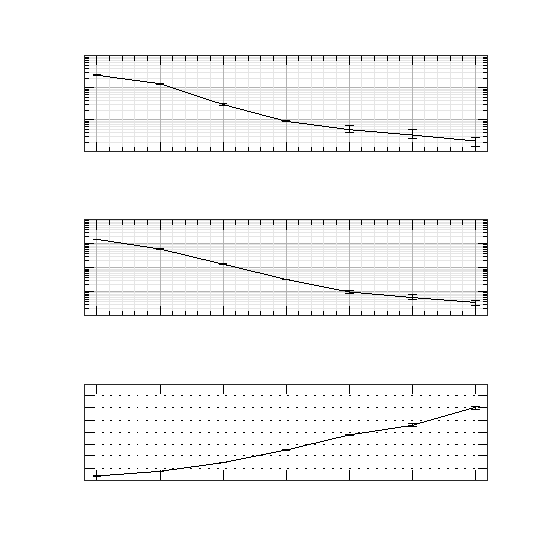
\includegraphics{./figures/parts/02/chapters/04/sections/04/uf_varying_resolution}}%
    \gplfronttext
  \end{picture}%
\endgroup
